\documentclass[conference,compsoc]{IEEEtran}

% *** CITATION PACKAGES ***
%
\ifCLASSOPTIONcompsoc
  % IEEE Computer Society needs nocompress option
  % requires cite.sty v4.0 or later (November 2003)
  \usepackage[nocompress]{cite}
\else
  % normal IEEE
  \usepackage{cite}
\fi

% *** PDF, URL AND HYPERLINK PACKAGES ***
%
\usepackage{url}
% url.sty was written by Donald Arseneau. It provides better support for
% handling and breaking URLs. url.sty is already installed on most LaTeX
% systems. The latest version and documentation can be obtained at:
% http://www.ctan.org/pkg/url
% Basically, \url{my_url_here}.

\usepackage{graphicx}
\usepackage{caption}
\usepackage{subcaption}
\usepackage{xcolor}
\usepackage{colortbl}
\usepackage{multirow}
%\usepackage[hyphens]{url}
\usepackage[hidelinks]{hyperref}
\usepackage[nolist]{acronym}
\usepackage{amssymb}
\usepackage{blindtext}
\usepackage{enumitem}
\usepackage{makecell}
\usepackage{listing}
\usepackage{tabularx}
\usepackage{enumitem} % Add labels for RQs defined in enumerated list
\usepackage{amsmath}
\usepackage{tikz}
\usetikzlibrary{positioning, fit} % positioning enables relative positions in tikz, fit enable to create groups of nodes

\definecolor{verylightgray}{RGB}{240,240,240}
\definecolor{fuchsia}{rgb}{1.0, 0.0, 1.0}

%% Tikz
\usepackage{tikz}
\usepackage{tikzscale}
\usepackage{pgfplots}
\DeclareUnicodeCharacter{2212}{−}
\usepgfplotslibrary{groupplots,dateplot}
\usetikzlibrary{patterns,shapes.arrows}
\pgfplotsset{compat=newest}

% correct bad hyphenation here
\hyphenation{op-tical net-works semi-conduc-tor}

\newcommand{\todo}[1]{{\color{red}\textbf{Todo: #1}}}
\newcommand{\new}[1]{{\color{blue}#1}}
%\newcommand{\footurl}[1]{{\footnote{\url{#1}}}}
\newcommand{\footurl}[1]{{\footnote{#1}}}

\newcommand{\jl}[1]{{\color{fuchsia}\textbf{Johannes:} #1}}
\newcommand{\lb}[1]{{\color{red}\textbf{Lars:} #1}}
\newcommand{\aw}[1]{{\color{green!60!black}\textbf{Anna:} #1}}

\newcommand{\checkNum}[1]{{\color{red}#1}}


\begin{document}
%
% paper title
% Titles are generally capitalized except for words such as a, an, and, as,
% at, but, by, for, in, nor, of, on, or, the, to and up, which are usually
% not capitalized unless they are the first or last word of the title.
% Linebreaks \\ can be used within to get better formatting as desired.
% Do not put math or special symbols in the title.
\title{An Empirical Study of Prevalence, Purpose, and Dangers\\ of Unsafe Go Code in the Wild}


% conference papers do not typically use \thanks and this command
% is locked out in conference mode. If really needed, such as for
% the acknowledgment of grants, issue a \IEEEoverridecommandlockouts
% after \documentclass

% for over three affiliations, or if they all won't fit within the width
% of the page (and note that there is less available width in this regard for
% compsoc conferences compared to traditional conferences), use this
% alternative format:
% 
\author{
\IEEEauthorblockN{
A A\IEEEauthorrefmark{2},
B B\IEEEauthorrefmark{1},
C C\IEEEauthorrefmark{1}, 
Mira Mezini\IEEEauthorrefmark{1}
}
\IEEEauthorblockA{
Technical University of Darmstadt, D-64289 Darmstadt, Germany\\
}
\IEEEauthorblockA{\IEEEauthorrefmark{1}
E-mail: \{A, B , C, mezini\}@cs.tu-darmstadt.de \\
}
\IEEEauthorblockA{\IEEEauthorrefmark{2}
E-mail: A@cs.tu-darmstadt.de \\
}
}

\newcommand{\toolUsage}{\textit{go-geiger}}
\newcommand{\toolSA}{\textit{go-safer}}
\newcommand{\unsafe}{\textit{unsafe}}

\newcommand{\projsAnalyzed}{\checkNum{343}}
\newcommand{\initalProjs}{\checkNum{500}}
\newcommand{\withoutModules}{\checkNum{150}}
\newcommand{\notCompiled}{\checkNum{7}}

% use for special paper notices
%\IEEEspecialpapernotice{(Invited Paper)}

% make the title area
\maketitle

% As a general rule, do not put math, special symbols or citations
% in the abstract
\begin{abstract}
The Go programming language aims to provide memory and thread safety through compile-time measures such as a strict type system that prevents invalid memory accesses and data races. However, it also offers a way of circumventing this safety net through using the \unsafe{} package.
This package allows arbitrary type casts and pointer arithmetic.
There are legitimate use cases, but such uses must be done with extreme caution to avoid introducing vulnerabilities common to C programs, like buffer overflows and use-after-free.
Furthermore, usages of \unsafe{} may be present not only in a project's first-party source code, but can be introduced through third-party dependencies as well.
In this work, we present \toolUsage{}, a novel tool for Go developers to count \unsafe{} usages in a package and its dependencies.
This tool enables developers to focus auditing efforts on the packages that actually contain \unsafe{} usages, therefore increasing cost and time efficiency.
Using \toolUsage{}, we contribute a large-scale quantitative study on the usage of \unsafe{} in the \projsAnalyzed{} most popular open-source Go projects on GitHub, including a manual analysis of \numberCodeSnippets{} code samples on how \unsafe{} is used and for what purpose.
We find that \percentagePackagesWithUnsafe{} of packages used transitively by the projects contain \unsafe{} usages. 
\percentageProjectsWithUnsafe{} of projects contain at least one usage that is not part of the standard library, and \percentageProjectsAndDependenciesUnsafe{} of projects contain at least one \unsafe{} in the project or one of its transitive dependencies.
The analyzed projects use \unsafe{} primarily for efficiency reasons and to create functionality of generics, which are not available in current versions of Go.
Based on the usage patterns found, we present dangers and possible exploit vectors. Finally, we present \toolSA{}, a novel static analysis tool to identify two dangerous and common usage patterns that were previously undetected with existing tools.

\end{abstract}

% no keywords

% For peer review papers, you can put extra information on the cover
% page as needed:
% \ifCLASSOPTIONpeerreview
% \begin{center} \bfseries EDICS Category: 3-BBND \end{center}
% \fi
%
% For peerreview papers, this IEEEtran command inserts a page break and
% creates the second title. It will be ignored for other modes.
\IEEEpeerreviewmaketitle


\section{Introduction}
\label{sec:intro}


The adoption of memory-safe languages for all kinds of different applications has been increasing significantly in the last decade. 
While environments and languages such as Java, Rust, Nim or Google's Go try to eliminate many bug classes through their language design and/or runtime, they also provide, to varying degrees, escape hatches to perform potentially unsafe operations if explicitly requested.
These might be used for optimization purposes, for convenience of the programmer, to directly access hardware or to circumvent limitations of the programming language.
Often enough unsafe code blocks are indirectly introduced through 3rd party libraries \cite{evans2020} and thus not directly obvious to the application developer.
Not knowing about the dangers introduced through external dependencies can have severe consequences.
Thus, developers and administrators need ways to quickly evaluate the potential risks introduced by other code.

For this paper we took a deeper look into Google's Go programming language and the usage of unsafe code blocks within the most popular software projects using it. 
During this work, we developed two specific tools for developers and security analysts. The first one, called \toolUsage{}, analyzes a project including its dependencies for general usage of unsafe and in which context.
The second one, called \toolSA{}, helps during development by providing meaningful hints to potentially dangerous usages of unsafe and how to avoid them. 
We analyzed the top \projsAnalyzed{} Go projects on GitHub to see how often unsafe is used in the wild. \aw{I would already mention some of our results here, e.g., We found that AB~\% of the applications make use of unsafe either in the application code or in a dependency.} 
From there we identified reasons for introducing unsafe in the source code in the first place and also whether it was really necessary.
Additionally, we provide insights into the dangers and possible exploit vectors to some of the patterns we found in the wild. 
Thus, we show the severe nature of these bugs.
Through the course of this work we made over \checkNum{14} pull requests to analyzed projects and libraries, fixing over \checkNum{60} individual potentially dangerous unsafe usages.

In this paper, we present the following contributions:

\begin{itemize}
\item We present to the best of our knowledge the first large-scale quantitative evaluation on the usage of unsafe in the \projsAnalyzed{} most popular Go projects on GitHub
\item We present a novel data set with \checkNum{1,400} labeled occurrences of unsafe code in various contexts of Go projects, providing insight into what is being done and for what purpose
\item We present novel evidence on how to exploit Go unsafe usages in the wild
\item We present a novel tool, \toolUsage{}, for detecting and scoring the presence of unsafe in Go projects and their dependencies
\item We present a novel static code analysis tool, \toolSA{}, to aid developers in identifying potentially problematic unsafe usage in their code base that were previously uncaught with existing tools
\end{itemize}

The paper is organized as follows:
Section~\ref{sec:background} gives a short introduction into unsafe Go.
Section~\ref{sec:rw} discusses related work. 
In Section~\ref{sec:impl}, we present our methodology and data selection for the large-scale study, as well as our approach to collect and label data.
Section~\ref{sec:eval} presents the results of our work.
Section~\ref{sec:exploits} presents potential exploit vectors to some unsafe patterns found in the wild.
In Section~\ref{sec:tools}, we present our novel tools \toolUsage{} and \toolSA{}.
Section~\ref{sec:discussion} discusses our approach, including potential threads to validity.
Section~\ref{sec:concl} concludes the paper and outlines areas of future work.

\section{Go's \unsafe{}~package}
\label{sec:background}



The Go programming language, like other memory-safe languages, provides the \unsafe{}~package\footnote{\url{https://golang.org/pkg/unsafe}}, which offers 
(a) the functions \textit{Sizeof}, \textit{Alignof}, and \textit{Offsetof} that are evaluated at compile time and provide access into memory alignment details of Go data types that are otherwise inaccessible, %unnecessary to know, and thus, inaccessible.
and (b) a pointer type, \textit{unsafe.Pointer} that allows developers to circumvent restrictions of regular pointer types.

One can cast any pointer to/from \textit{unsafe.Pointer}, thus enabling casts between completely arbitrary types, as illustrated in  
%
%In the remainders of this section, we discuss two example use cases of the \unsafe{} package in practice. 
Listing~\ref{lst:unsafe-ex-in-place-cast}.
%shows the usage of the \unsafe{} package to cast between arbitrary types.
In this example, \textit{in.Items} is assigned to a new type (\textit{out.Items}) in line 3 without reallocation for efficiency reasons.\footnote{This code was taken from the Kubernetes \textit{k8s.io/apiserver} module with minor adjustments.} 
Furthermore, casts between \textit{unsafe.Pointer} and \textit{uintptr} are also enabled, mainly for pointer arithmetic.
A \textit{uintptr} is an integer type with a length sufficient to store memory addresses. 
However, it is not a pointer type, hence, not treated as a reference.
%The first \textit{unsafe.Pointer} rule allows casts between completely arbitrary types, and the latter one allows the use of pointer arithmetic.
%The usage of the \unsafe{}~package removes the safety net provided by the Go type system and compiler, and brings developers down to the flexibility and danger of the pointers in C.
%
Listing~\ref{lst:unsafe-ex-escape-analysis} presents an example of casts involving \textit{uintptr}. 
%The code is taken from the \textit{modern-go/reflect2} module.
In Line 2, the \textit{unsafe.Pointer} is converted to \textit{uintptr}.
Thus, the memory address is stored within a non-reference type.
Hence, the back-conversion in Line 3 causes the \textit{unsafe.Pointer} to be hidden for the \textit{escape analysis (EA)} that Go's garbage collector uses 
%manages the memory allocations and tries to identify memory which can be freed up.
%For this task, it uses \textit{escape analysis (EA)} 
to determine whether a pointer is local to a function and can be stored in the corresponding stack frame, 
or whether it can \textit{escape} the function and needs to be stored on the heap \cite{wang2020}. 
Since \textit{uintptr} values are not pointer types, storing the address of a pointer in a variable of such a type and then converting it back causes the \textit{EA} to miss the chain of references to the underlying value in memory. 
Therefore, Go will assume a value does not escape when it actually does, and may place it on the stack.
Correctly used it can improve efficiency because deallocation is faster on the stack than on the heap~\cite{wang2020}.
However, used incorrectly it can cause security problems as shown later in Section~\ref{sec:appr}.

\begin{lstlisting}[language=Golang, label=lst:unsafe-ex-in-place-cast, caption=In-place cast using the \unsafe{} package
from the Kubernetes \textit{k8s.io/apiserver} module with minor changes.
,float, belowskip=-1.5em]
func autoConvert(in *PolicyList, out *audit.PolicyList) error {
	// [...]
	out.Items = *(*[]audit.Policy)(unsafe.Pointer(&in.Items))
	return nil
}
\end{lstlisting}

\begin{lstlisting}[language=Golang, label=lst:unsafe-ex-escape-analysis, caption=Hiding a value from escape analysis from the \textit{modern-go/reflect2} module.
, float, belowskip=-1.5em]
func NoEscape(p unsafe.Pointer) unsafe.Pointer {
	x := uintptr(p)
	return unsafe.Pointer(x ^ 0)
}
\end{lstlisting}


% \subsection{Go Dependency Management}

%Old way: packages, Go Path

%New way: modules, registries, \textit{go.mod} file.

%Package cache, versions, bad reproducibility, relatively high error rates for dependency resolution.

\section{Related Work}
\label{sec:rw}

\cite{alnaeli2017, evans2020, qin2020, pashchenko2018, watanabe2017, smith2020}
\section{Methodology and Implementation}
\label{sec:impl}

The goal of our study is to understand how \unsafe{}~is used in open-source projects and the implications on the security of Go applications. 
To achieve this aim, we answer the following research questions:

\begin{enumerate}[label={RQ\arabic*},leftmargin=*] 
    \item How many projects use \unsafe{} in Go code in their application? \label{rq:prevalApp}
    \item How many projects introduce \unsafe{} through their dependencies, and from which registries? \label{rq:prevalDeps}
    \item How deep in the import stack are the most imported \unsafe{} code packages? \label{rq:depsDepth}
    \item Which \unsafe{} keywords are used most? \label{rq:distTypes}
    \item What \unsafe{} operations are used in practice, and what is their goal? \label{rq:purpose}
    \item Are there problems arising from the use of \unsafe{} that can lead to exploitable vulnerabilities? \label{rq:probsUnsafe}
\end{enumerate}

Later ref to the RQ with the label \ref{rq:probsUnsafe}.

\subsection{Data Set Creation}

To answer our research question, we create a data set of open-source Go code available on GitHub.
As our research is focused on projects, we decide to crawl the \initalProjs{} most-stared Go projects available on GitHub. 
To further understand the influence of the dependencies, we selected the applications supporting \textit{go modules}.
With the introduction of Go \checkNum{1.13}, \textit{go modules} are the way to include dependencies within a Go application with the help of the Go toolchain. 
Unfortunately, \withoutModules{} of the projects did not yet support go modules and we had to exclude them.
We further, had to remove \notCompiled{} projects as we couldn't compile those.
As a result, we end up with \projsAnalyzed{} top-rated Go projects collected from GitHub. 

\aw{Perhaps, we want to include some star stats or similar stats to show that we have relevant Go projects.}


\begin{figure*}[!t]
    \begin{tikzpicture}
        % Define tikz styles
        \tikzset{metaGroup/.style={
            draw = gray, thin, rounded corners,
        }}
        \tikzset{inner/.style={
            font=\tiny,
        }}
    
        % create nodes
        \node (mark) {\includegraphics[width=11mm]{gfx/figures/mark.png}};
        \node (checkout) [right=of mark, yshift=10mm, inner] {\initalProjs};
        \node (goModules) [right= of mark, inner] {- \withoutModules{}};
        \node (compile) [right=of mark, yshift=-10mm, inner] {- \notCompiled{}};
        \node (projects) [fit=(checkout)(goModules)(compile)] {};
        \node (dataSet) [fit=(projects)(mark), metaGroup, label=Data set creation] {};
        
        \node (analysis) [right=of dataSet] {analysis};
        
        % create connections between components
        \draw [->] (mark) -- (projects);
        \draw [->, thin, font=\tiny] (checkout) -- node[anchor=east] {no go modules} (goModules);
        \draw [->, thin, font=\tiny] (goModules) -- node[anchor=east] {not build} (compile);
        
        \draw [->] (dataSet) -- node[anchor=south] {\projsAnalyzed} (analysis);
    \end{tikzpicture}
    \caption{Overview of our Methodology and Empirical Results.}
    \label{fig:overview}
\end{figure*}


\section{Study Results}
\label{sec:eval}

\begin{figure}[ht]
    \centering
    \includegraphics[width=0.5\textwidth]{gfx/figures/distribution-unsafe-types.png}
    \caption{Distribution of different types of unsafe token types. Answers \ref{rq:distTypes}}
    \label{fig:unsafe-tokens-distribution}
\end{figure}

\begin{figure*}[ht]
    \centering
    {\scriptsize \includegraphics[width=\textwidth,height=6cm]{gfx/figures/unsafe-import-depth.tikz}}
    \caption{Import Depth of Unsafe Packages. Answers \ref{rq:depsDepth}: unsafe packages are around \checkNum{3.5 $\pm 2$} hops away, thus manageable to find manually. \jl{Add mean and deviation}}
    \label{fig:unsafe-import-depth}
\end{figure*}

\begin{figure*}[ht]
    \centering
    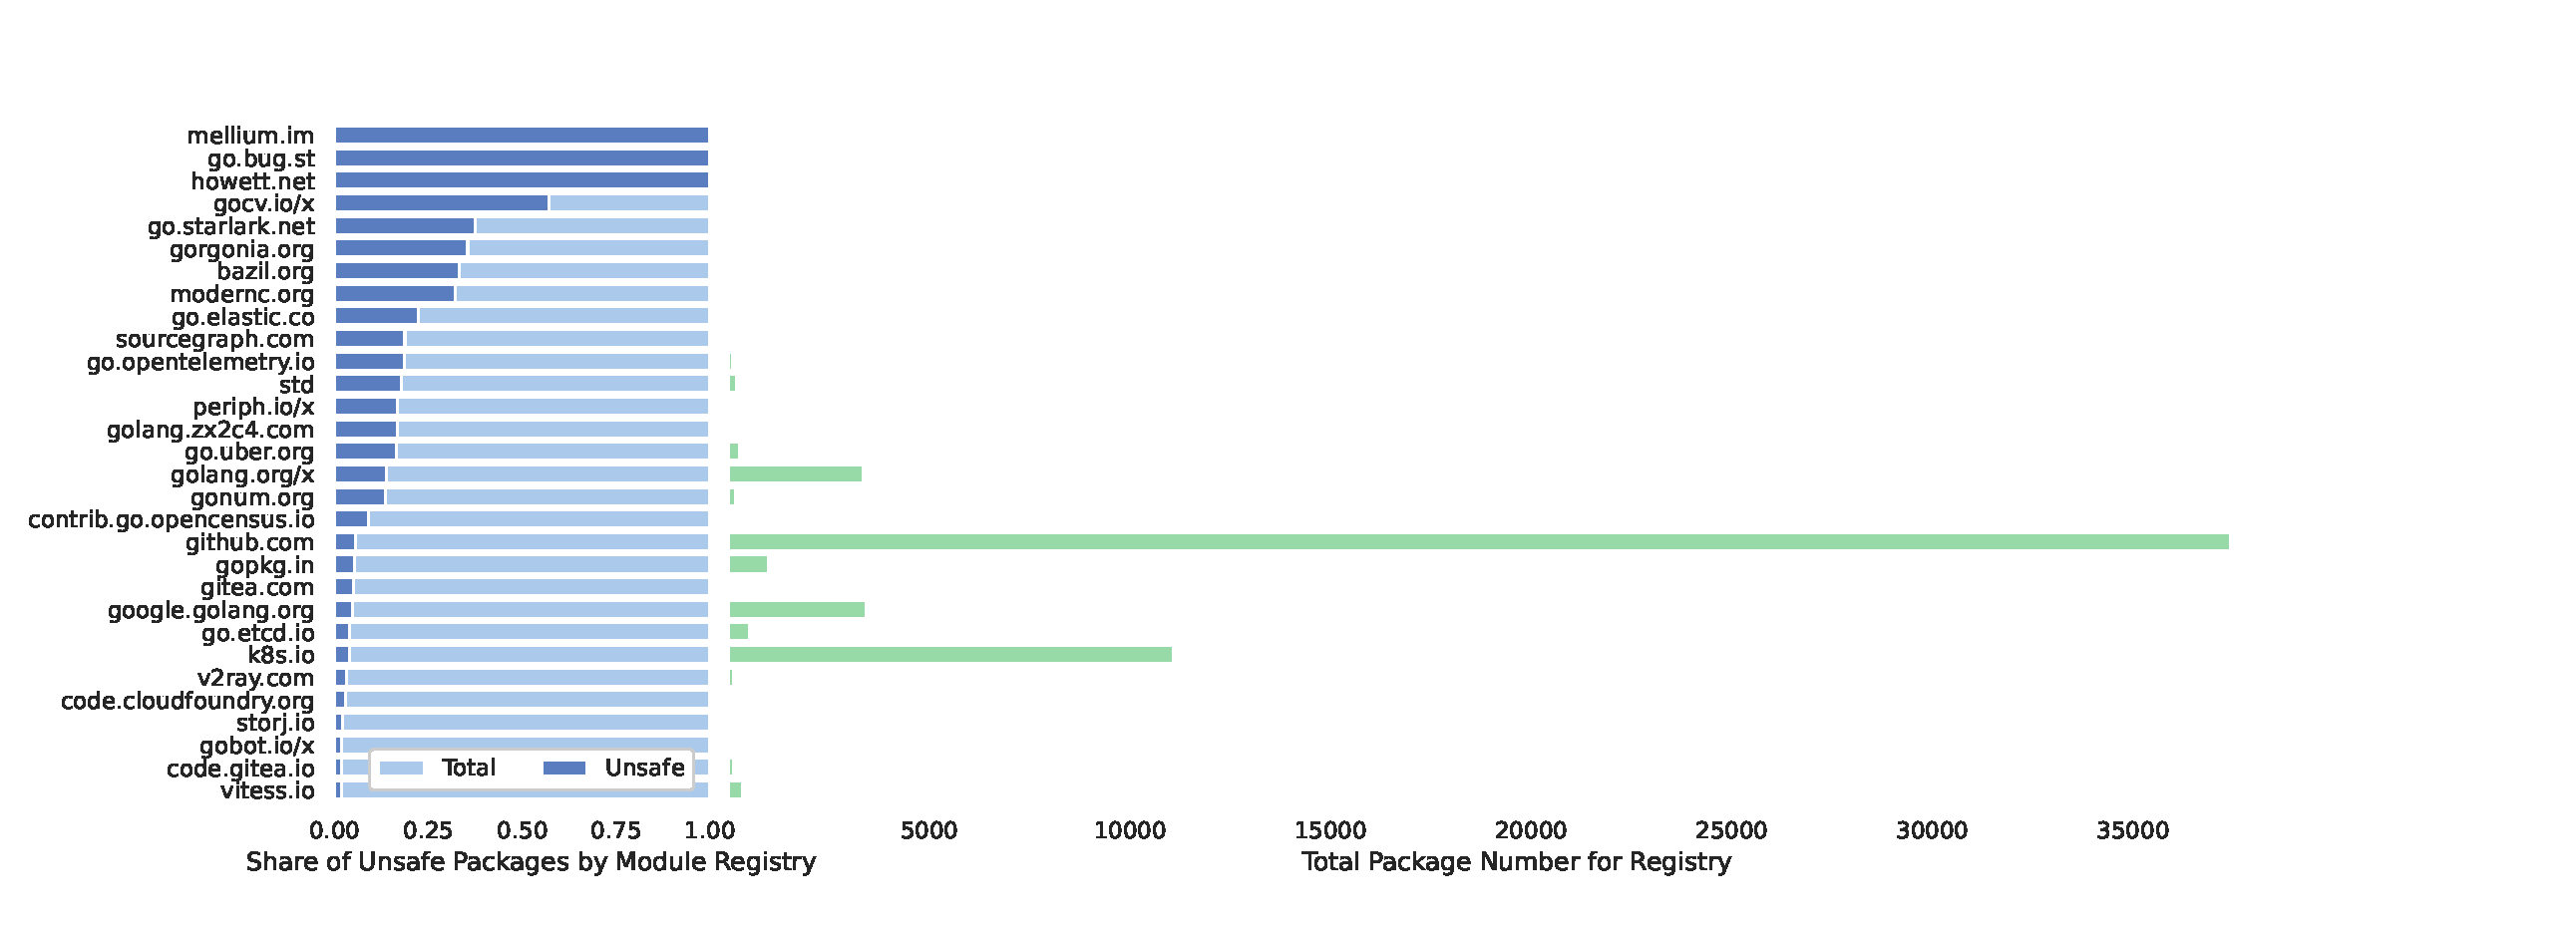
\includegraphics[width=\textwidth]{gfx/figures/unsafe-packages-by-registry-n30.eps}
    \caption{Share of Unsafe Packages by Registry along with Total Package Count for Registries, Showing the Top \checkNum{30} Registries by Unsafe Share. Answers \ref{rq:prevalDeps} in its current form}
    \label{fig:unsafe-by-registry}
\end{figure*}

\begin{table}[h]
    \centering
    \caption{Selected projects for creation of the labeled data set}
    \label{tbl:dataset-projects}
    \begin{tabular}{llrrll}
    \hline
        {}  &                                               Name &  Stars &  Forks &   Revision \\ \hline
        1   &                              kubernetes/kubernetes &  66512 &  23806 &  fb9e1946b0 \\
        2   &                       mattermost/mattermost-server &  18277 &   4157 &  e83cc7357c \\
        3   &                                    rancher/rancher &  14344 &   1758 &  56a464049e \\
        4   &                                   weaveworks/scope &   4354 &    554 &  bf90d56f0c \\
        5   &                                          rook/rook &   7208 &   1472 &  ff90fa7098 \\
        6   &                                      elastic/beats &   8852 &   3207 &  df6f2169c5 \\
        7   &                                hashicorp/terraform &  22151 &   5729 &  01f91316da \\
        8   &                                      cilium/cilium &   5501 &    626 &  9b0ae85b5f \\
        9   &                                       grafana/loki &   9537 &    922 &  10a1f28a85 \\
        10  &                                  gorgonia/gorgonia &   3373 &    301 &  5fb5944d4a \\
        \hline
    \end{tabular}
\end{table}

\begin{table*}[t]
    \centering
    \caption[Labeled unsafe.Pointer usages in application code samples Answers \ref{rq:purpose}]%
    {Labeled unsafe.Pointer usages in application code samples \newline \tiny ~ \newline \small
        \underline{eff}: efficiency, \underline{gen}: generics, \underline{ser}: (de)serialization,
        \underline{inev}: inevitable use, \underline{SR}: safer reflections, \underline{LC}: layout control,
        \underline{EA}: hide from escape analysis, \underline{UU}: unused,
        \underline{doc}: documentation \newline \tiny ~}
    \label{tbl:dataset-classes-app}
    \begin{tabular}{r|ccccccccc|r}
                                          &  eff &  gen & ser & inev &  SR &  LC &  EA &  UU & doc &  {}   \\ \hline
                 conversion-struct-struct &  396 &   58 &   7 &    2 &   2 &   1 &    &     &     &   466 \\
        \rowcolor{verylightgray}
                  conversion-struct-basic &   80 &   35 &   5 &      &     &   1 &    &     &     &   121 \\
                        conversion-header &   26 &    8 &   3 &      &     &     &    &     &     &    37 \\
        \rowcolor{verylightgray}
                  conversion-struct-bytes &   21 &    1 &  70 &    1 &     &   3 &    &     &     &    96 \\
                     direct-memory-access &    9 &   19 &     &    9 &   1 &   1 &    &     &     &    39 \\
        \rowcolor{verylightgray}
                       pointer-arithmetic &    7 &    2 &   1 &      &     &   7 &  1 &     &     &    18 \\
                           data-structure &    7 &    5 &     &    2 &  22 &   1 &    &   1 &     &    38 \\
        \rowcolor{verylightgray}
                                 delegate &    4 &   63 &   1 &   19 &   1 &     &    &     &     &    88 \\
                          type-reflection &      &   32 &     &      &   2 &     &    &     &     &    34 \\
        \rowcolor{verylightgray}
                                  syscall &      &      &     &   21 &     &     &    &     &     &    21 \\
                                   unused &      &      &     &      &     &     &    &  15 &     &    15 \\
        \rowcolor{verylightgray}
                                  comment &      &      &     &      &     &     &    &  23 &   4 &    27 \\ \hline
                                       {} &  550 &  223 &  87 &   54 &  28 &  14 &  1 &  39 &   4 &  1000 \\
    \end{tabular}
\end{table*}

\begin{table*}[t]
    \centering
    \caption[Labeled unsafe.Pointer usages in standard library samples. Answers \ref{rq:purpose}]%
        {Labeled unsafe.Pointer usages in standard library samples \newline \tiny ~ \newline \small
            \underline{no GC}: avoid garbage collector, \underline{typ}: types implementation,
            \underline{mem}: memory management, \underline{inev}: inevitable use, \underline{eff}: efficiency,
            \underline{ser}: (de)serialization, \underline{LC}: layout control, \underline{cgo}: CGo mechanics,
            \underline{EA}: hide from escape analysis, \underline{UU}: unused, \underline{UU}: unnecessary use \newline \tiny ~}
    \label{tbl:survey-small-results-std}
    \begin{tabular}{r|ccccccccccc|r}
                                          & no GC & typ & mem & inev & eff & ser & LC & cgo & EA & UN & UU &   {} \\ \hline
                                  syscall &   151 &     &     &    3 &     &     &    &     &    &  1 &    &  155 \\
        \rowcolor{verylightgray}
                     direct-memory-access &       &  10 &  13 &      &  17 &   2 &  2 &     &    &    &    &   44 \\
                       pointer-arithmetic &       &   9 &   7 &    2 &   5 &     &  4 &   1 &  1 &    &    &   29 \\
        \rowcolor{verylightgray}
                 conversion-struct-struct &       &  20 &   4 &    4 &   1 &   9 &    &   1 &  1 &    &    &   40 \\
                  conversion-struct-basic &       &     &   3 &    1 &     &   2 &  2 &   1 &    &    &    &    9 \\
        \rowcolor{verylightgray}
                        conversion-header &       &   2 &   1 &      &     &     &    &     &    &    &    &    3 \\
                  conversion-struct-bytes &       &     &     &      &   4 &   8 &    &     &    &    &    &   12 \\
        \rowcolor{verylightgray}
                           data-structure &       &   7 &  11 &    1 &     &     &    &   3 &    &    &    &   22 \\
                                 delegate &       &   4 &  16 &   47 &     &     &    &     &  6 &    &    &   73 \\
        \rowcolor{verylightgray}
                          type-reflection &       &   3 &     &      &     &   1 &    &     &    &    &    &    4 \\
                                   unused &       &     &     &      &     &     &    &     &    &    &  8 &    8 \\
        \rowcolor{verylightgray}
                                  comment &       &     &     &      &     &     &    &     &    &    &  1 &    1 \\ \hline
                                       {} &   151 &  55 &  55 &   58 &  27 &  22 &  8 &   6 &  8 &  1 &  9 &  400 \\
    \end{tabular}
\end{table*}

\textbf{Answers to research questions:}

\checkNum{3355} of \checkNum{61839} (\checkNum{5.43\%}) transitively imported packages use unsafe. This answers \ref{rq:prevalDeps}

Number of projects: \checkNum{343}

Projects with $\geq 1$ unsafe project package: \checkNum{131} (\checkNum{38.19\%})

Projects with $\geq 1$ unsafe dependency: \checkNum{299} (\checkNum{87.17\%})

Projects with $\geq 1$ unsafe anywhere: \checkNum{312} (\checkNum{90.96\%})

These answer \ref{rq:prevalApp} and \ref{rq:prevalDeps}.

\section{Exploit Proof of Concepts}
\label{sec:exploits}

\section{Tools to Help Developers}
\label{sec:tools}

\aw{Why not discuss this in related work?}
\section{Discussion}
\label{sec:discussion}

\begin{itemize}
    \item exploit-ability is not only of academic nature
\end{itemize}

\input{09_conclusion}

% conference papers do not normally have an appendix

% use section* for acknowledgment
\ifCLASSOPTIONcompsoc
  % The Computer Society usually uses the plural form
  \section*{Acknowledgments}
\else
  % regular IEEE prefers the singular form
  \section*{Acknowledgment}
\fi

\input{10_acks}


% trigger a \newpage just before the given reference
% number - used to balance the columns on the last page
% adjust value as needed - may need to be readjusted if
% the document is modified later
%\IEEEtriggeratref{8}
% The "triggered" command can be changed if desired:
%\IEEEtriggercmd{\enlargethispage{-5in}}

% references section

% can use a bibliography generated by BibTeX as a .bbl file
% BibTeX documentation can be easily obtained at:
% http://mirror.ctan.org/biblio/bibtex/contrib/doc/
% The IEEEtran BibTeX style support page is at:
% http://www.michaelshell.org/tex/ieeetran/bibtex/
\bibliographystyle{IEEEtran}
% argument is your BibTeX string definitions and bibliography database(s)
\bibliography{IEEEabrv,references}

% that's all folks
\end{document}
